
\documentclass[class=report,crop=false]{standalone}
\usepackage[screen]{../exo7book}

\begin{document}

%====================================================================
\chapitre{La chaînette}
%====================================================================

\insertvideo{1qoruh8ADy4}{partie 1. Le cosinus hyperbolique}

\insertvideo{BlSRn3kWUNI}{partie 2. \'Equation de la chaînette}

\insertvideo{T-gUVEs51-c}{partie 3. Longueur d'une chaînette}



\section*{Introduction}



\begin{minipage}{0.49\textwidth}
La \defi{chaînette} est le nom que porte la courbe obtenue en tenant 
une corde (ou un collier, un fil,\ldots) par deux extrémités.
Sans plus tarder voici l'équation d'une chaînette :
$$y = a \ch\left( \frac x a \right)$$  
\end{minipage}
\begin{minipage}{0.5\textwidth}
\myfigure{0.9}{
\tikzinput{fig_chainette03}
}  
\end{minipage}


Ici <<$\ch$>> désigne le cosinus hyperbolique, défini à partir de la fonction exponentielle :
$y(x) = \frac a 2 \left( e^{\frac x a} + e^{-\frac x a} \right),$
 nous y reviendrons.


Le paramètre $a$ dépend de la chaînette : on peut écarter plus ou moins les mains.
Ou, ce qui revient au même, si l'on garde les mains fixes, on peut prendre des cordes de différentes longueurs.

C'est donc une courbe que vous voyez tous les jours :
la chaîne qui pend à votre cou ou le fil électrique entre deux pylônes.
Mais on le retrouve dans des endroits plus surprenants : 
vous pouvez voir des chaînettes avec des films de savon. 
Trempez deux cercles métalliques parallèles dans de l'eau savonneuse.
Il en sort une surface de révolution dont le profil est une chaînette.
Enfin, si vous souhaitez faire une arche qui s'appuie sur deux piles 
alors la forme la plus stable est une chaînette renversée.
Gaudi a beaucoup utilisé cette forme dans les bâtiments
qu'il a construits.

\bigskip

{\centering
  \hspace*{-1.3cm}
  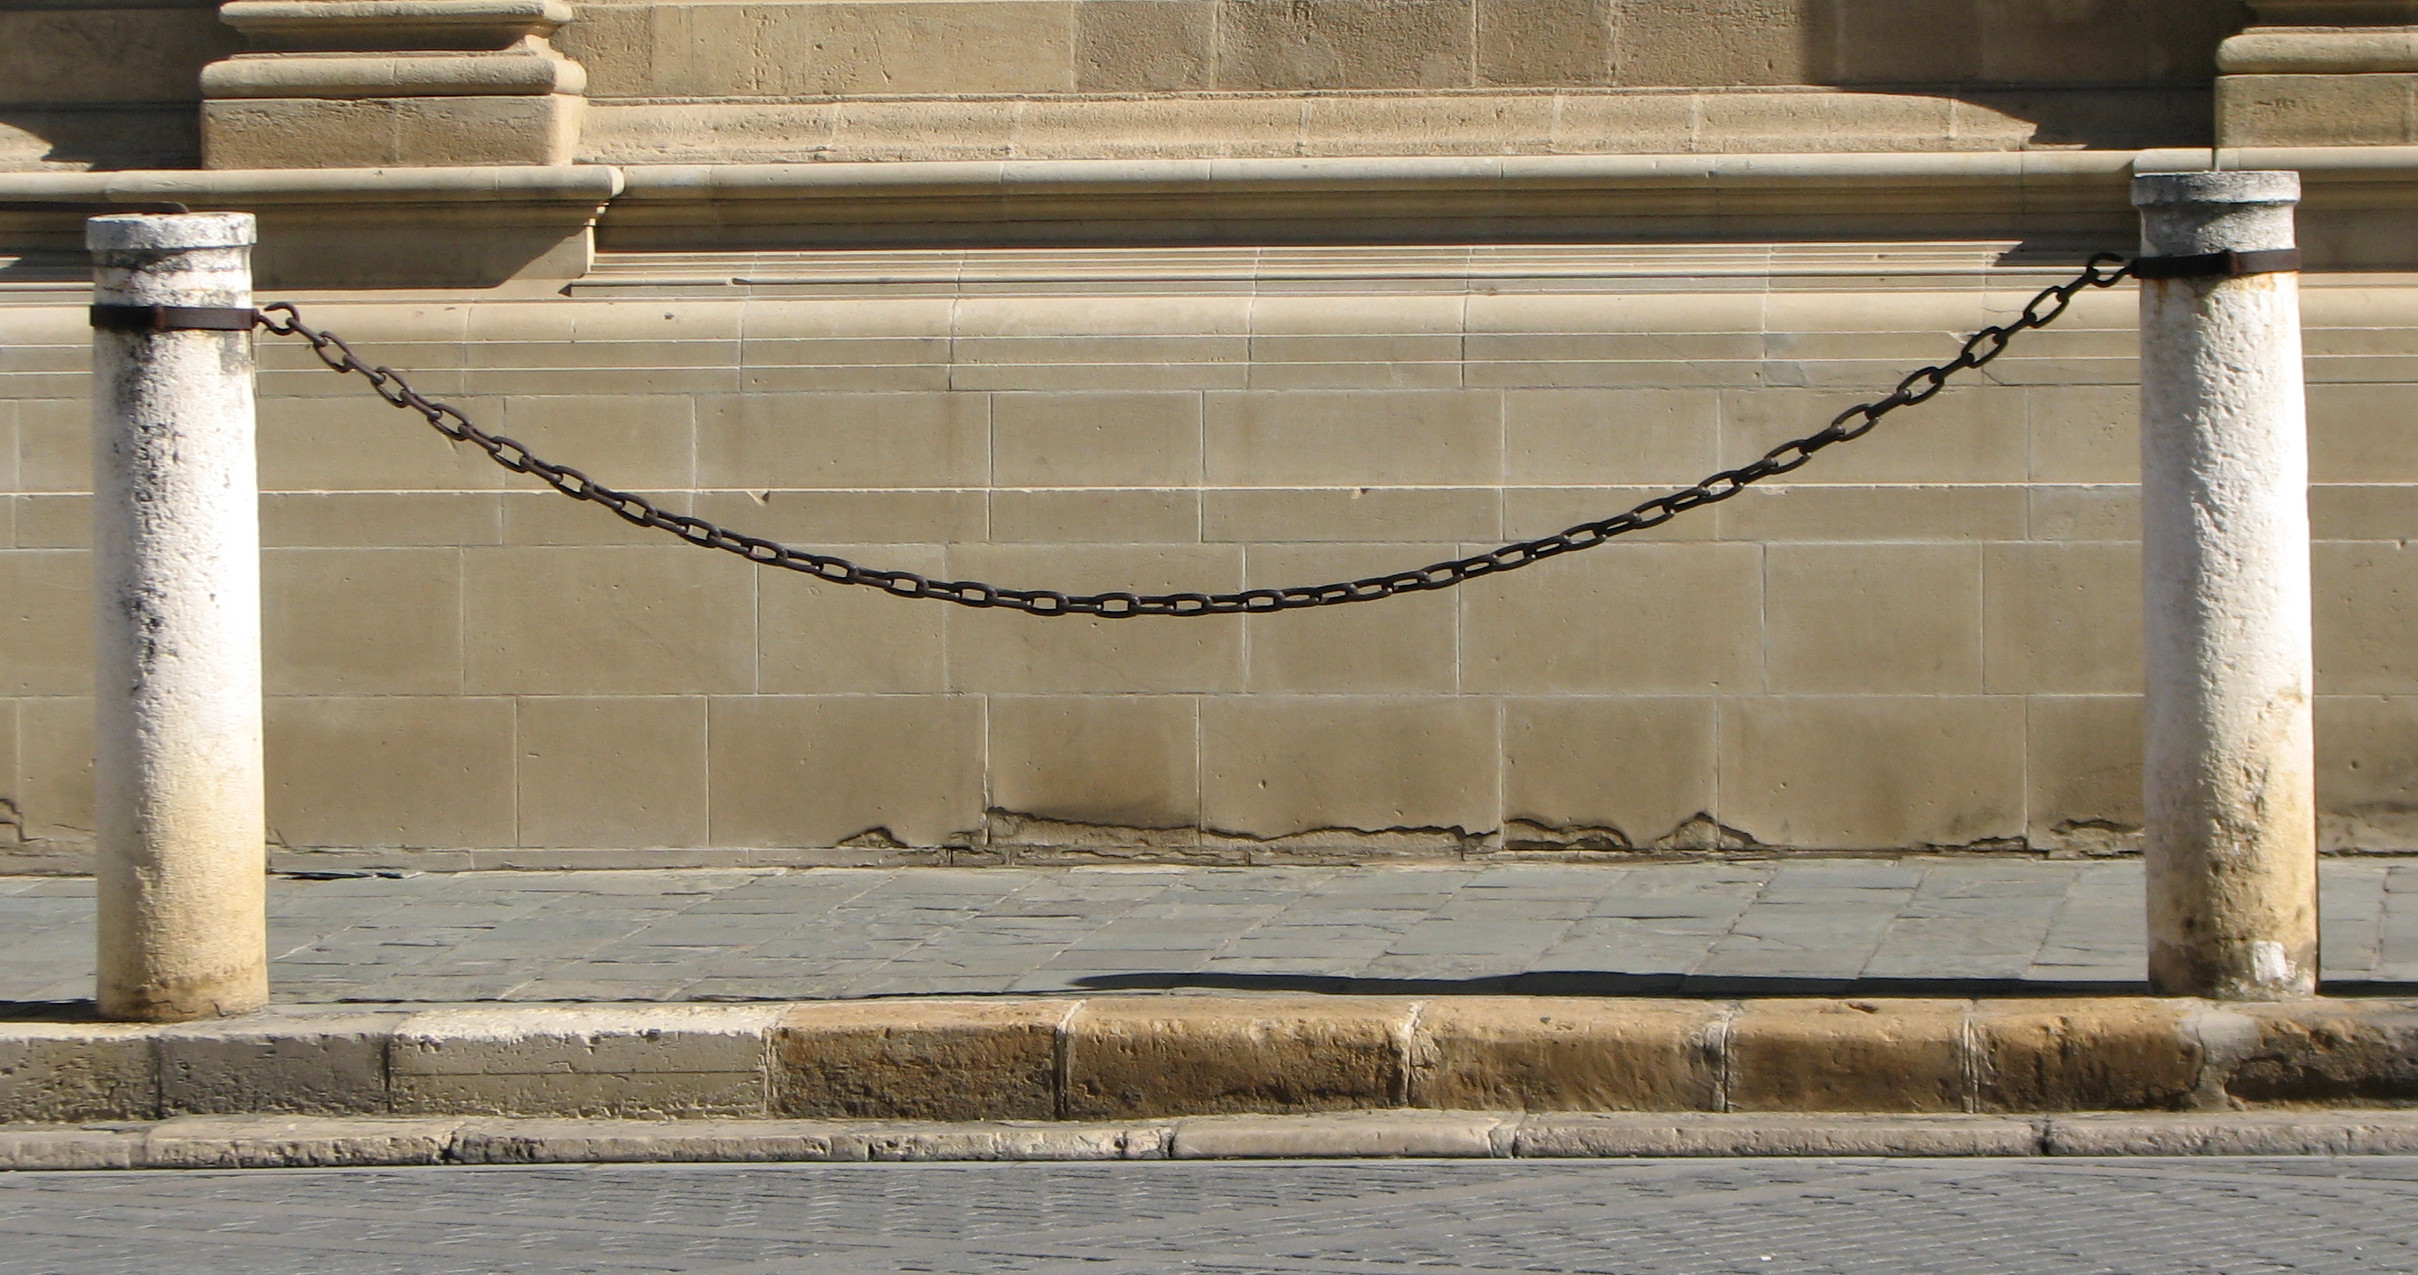
\includegraphics[height=4cm]{figures/Chainette_by_fdecomite.jpg} 
  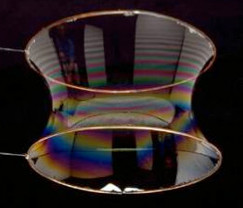
\includegraphics[height=4cm]{figures/Bulle_Savon_by_soapbubble.jpg} 
  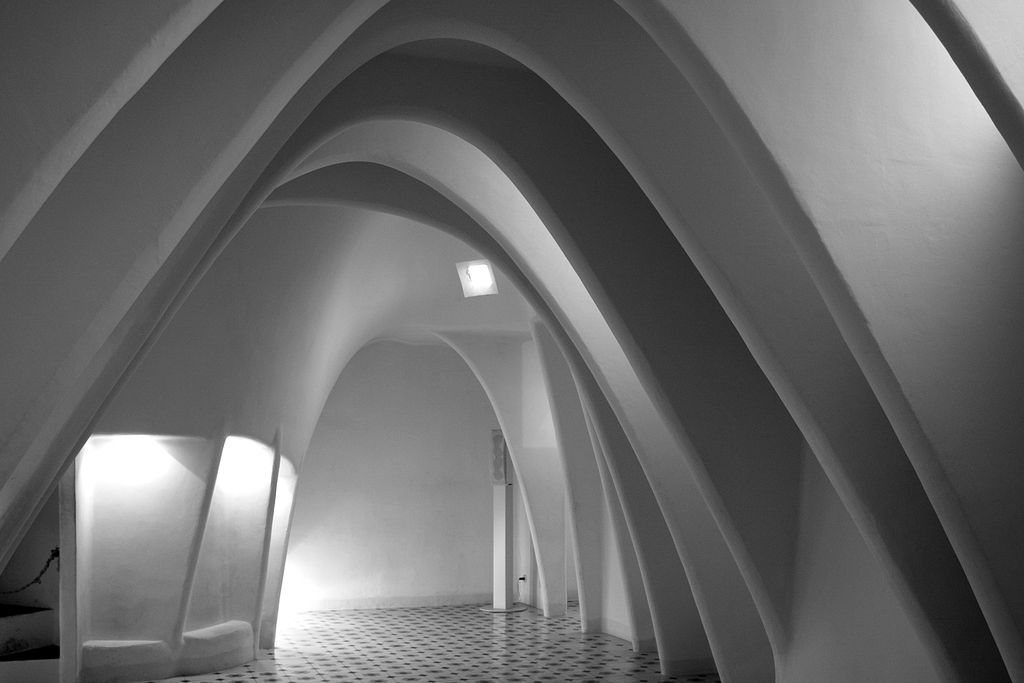
\includegraphics[height=4cm]{figures/Gaudi_by_Naveen_Jamal.jpg} 
}

\bigskip

Pour finir sur un bateau, si une voile rectangulaire est maintenue par deux
mats horizontaux et que le vent souffle perpendiculairement 
alors le profil de la voile est une chaînette. 

Stop ! Place aux maths : nous allons expliquer comment calculer l'équation d'une chaînette.





%%%%%%%%%%%%%%%%%%%%%%%%%%%%%%%%%%%%%%%%%%%%%%%%%%%%%%%%%%%%%%%%%%%%%%%%%%%%%%%%%%%%%%%%
\section{Le cosinus hyperbolique}

%---------------------------------
\subsection{Définition}

Le \defi{cosinus hyperbolique} et le \defi{sinus hyperbolique} sont la partie paire et impaire de l'exponentielle :
$$\ch x = \frac{e^x + e^{-x}}{2}, \qquad \sh x = \frac{e^x - e^{-x}}{2}.$$
\myfigure{1}{
\tikzinput{fig_chainette02}
\qquad
\tikzinput{fig_chainette01}
}


Voici quelques propriétés dont nous aurons besoin :
\begin{proposition}
\label{prop:chainette1}
\begin{enumerate}
 \item $\ch^2 x - \sh^2 x = 1$, pour tout $x \in \Rr$.
 \item $\ch ' x = \sh x$ et $\sh' x = \ch x$.
\end{enumerate}
\end{proposition}

\begin{remarque*}
Le nom cosinus hyperbolique et sinus hyperbolique ne sont pas un hasard :
souvenez-vous des formules d'Euler pour le cosinus et sinus classiques (dits aussi <<circulaires>>) :
$$\cos x = \frac{e^{\ii x} + e^{-\ii x}}{2}, \qquad \sin x = \frac{e^{\ii x} - e^{-\ii x}}{2\ii}.$$
L'analogie avec la définition de $\ch x$ et $\sh x$ justifie les termes <<cosinus>> et <<sinus>>. 
Reste à justifier le terme <<hyperbolique>>.
\myfigure{1}{
\tikzinput{fig_chainette04}
\qquad
\tikzinput{fig_chainette05}
}
Si nous dessinons une courbe paramétrée par $(x(t) = \cos t,y(t) = \sin t)$ alors
$x(t)^2+y(t)^2 = \cos^2 t + \sin^2 t =1$. Donc nous avons affaire à un cercle
(d'où le terme <<circulaire>>). 
Par contre si on dessine une courbe paramétrée par $(x(t) = \ch t, y(t) = \sh t)$.
Alors $x(t)^2 - y(t)^2 = \ch^2 t - \sh^2 t = 1$.
C'est l'équation d'une branche d'hyperbole ! 
\end{remarque*}

%---------------------------------
\subsection{Fonctions réciproques}

\begin{proposition}
\label{prop:chainette2}
\begin{itemize}
  \item La fonction $x \mapsto \ch x$ est une bijection
de $[0,+\infty[$ dans $[1,+\infty[$. Sa bijection réciproque est 
notée $\Argch x$. Donc :
$$\ch\big(\Argch(x)\big) = x  \quad \forall x \in [1,+\infty[ 
\qquad\qquad  \Argch\big(\ch(x)\big) = x
\quad   \forall x \in [0,+\infty[$$

  \item  La fonction $x \mapsto \sh x$ est une bijection
de $\Rr$ dans $\Rr$. Sa bijection réciproque est 
notée $\Argsh x$. Donc :
$$\sh\big(\Argsh(x)\big) = x  \qquad\qquad  \Argsh\big(\sh(x)\big) = x
\quad   \forall x \in \Rr$$

\end{itemize}
\end{proposition}

\shorthandoff{:}
\myfigure{1}{
\tikzinput{fig_chainette06}
\qquad
\tikzinput{fig_chainette07}
}
\shorthandon{:}

\bigskip

Pour résoudre une équation différentielle nous aurons besoin de la dérivée
de $\Argsh x$.
\begin{proposition}
\label{prop:chainette3}
Les fonctions $x \mapsto \Argch x$ et $x \mapsto \Argsh x$
sont dérivables et 
$$\Argch' x = \frac{1}{\sqrt{x^2-1}} \qquad\qquad \Argsh' x = \frac{1}{\sqrt{x^2+1}}.$$
\end{proposition}


%---------------------------------
\subsection{Expression logarithmique}

En fait, les fonctions hyperboliques inverses peuvent s'exprimer à l'aide 
des fonctions usuelles :
\begin{proposition}
\label{prop:chainette4}
$$\Argch x  =  \ln\left( x+\sqrt{x^2-1} \right), \quad \text{ pour } x\ge1.$$
$$\Argsh x  =  \ln\left( x+\sqrt{x^2+1} \right), \quad \text{ pour } x \in \Rr.$$
\end{proposition}


%---------------------------------
\subsection{Les démonstrations}

Nous donnons les preuves des propositions précédentes pour la fonction cosinus hyperbolique.
Les formules pour le sinus hyperbolique s'obtiennent de façon similaire.

\begin{proof}[Preuve de la proposition \ref{prop:chainette1}]
\begin{enumerate}
  \item $\ch^2 x- \sh^2 x = \frac14 \big[ (e^x+e^{-x})^2 - (e^x-e^{-x})^2 \big] = 
 \frac14 \big[ (e^{2x}+2+e^{-2x}) - (e^{2x}-2+e^{-2x})  \big] = 1$.

  \item $\frac{d}{dx}(\ch x) = \frac{d}{dx} \frac{e^x+e^{-x}}{2} = \frac{e^x-e^{-x}}{2}  = \sh x$.
\end{enumerate}
  
\end{proof}


\begin{proof}[Preuve de la proposition \ref{prop:chainette2}]
\'Etudions la restriction de la fonction $\ch : [0,+\infty[ \to [1,+\infty[$.
\begin{itemize}
  \item Comme $\ch' x = \sh x \ge 0$, pour $x\ge 0$, alors la restriction de la fonction $\ch$ est croissante.
  Elle est même strictement croissante (la dérivée ne s'annule qu'en $0$).
  
  \item Comme $\ch 0 =1$, que $\ch x \to +\infty$ lorsque $x \to +\infty$,
  alors par continuité et la stricte croissance, la restriction $\ch : [0,+\infty[ \to [1,+\infty[$
  est une bijection.
\end{itemize}
Par définition, la bijection réciproque de cette restriction est $\Argch x : [1,+\infty[ \to [0,+\infty[$
et vérifie :
$$\Argch\big(\ch x\big) = x \qquad \text{ pour tout } x \in [0,+\infty[$$
$$\ch\big(\Argch x\big) = x \qquad \text{ pour tout } x \in [1,+\infty[.$$
\end{proof}


\begin{proof}[Preuve de la proposition \ref{prop:chainette3}]
Comme la fonction $x \mapsto \ch'x$  ne s'annule pas sur $]0,+\infty[$
alors la fonction $\Argch$ est dérivable sur $]1,+\infty[$.
On calcule la dérivée par dérivation de l'égalité $\ch(\Argch x) = x$ :
$$\Argch' x \cdot \sh(\Argch x) = 1$$
puis on utilise l'identité $\ch^2 u - \sh^2 u = 1$ avec $u = \Argch x$ :
$$\Argch' x = \frac{1}{\sh(\Argch x)} = \frac{1}{\sqrt{\ch^2(\Argch x)-1}}
= \frac{1}{\sqrt{x^2-1}}.$$  
\end{proof}


\begin{proof}[Preuve de la proposition \ref{prop:chainette4}]
Notons $f(x)=\ln\big(x+ \sqrt{x^2+1}\big)$. 
   $$f'(x) = \frac{1+\frac{x}{\sqrt{x^2+1}}}{x+ \sqrt{x^2+1}} = \frac{1}{\sqrt{x^2+1}} = \Argsh' x.$$ 
  Comme de plus $f(0)=\ln(1)=0$ et $\Argsh 0 = 0$ (car $\sh 0 = 0$), on en déduit que pour tout
  $x\in \Rr$, $f(x) = \Argsh x$.
\end{proof}


%%%%%%%%%%%%%%%%%%%%%%%%%%%%%%%%%%%%%%%%%%%%%%%%%%%%%%%%%%%%%%%%%%%%%%%%%%%%%%%%%%%%%%%%
\subsection{Dérivée des physiciens, dérivée des mathématiciens}

Deux notations pour la dérivée s'affrontent : celle du mathématicien $f'(x)$
et celle du physicien $\frac{df}{dx}$. Comparons-les.
La dérivée de $f$ en $x$ est par définition la limite (si elle existe) du taux d'accroissement :
$$\frac{f(x+h)-f(x)}{x+h-x},$$
lorsque $h$ tend vers $0$.
Notons $h = dx$ et $df = f(x+h)-f(x) = f(x+dx)-f(x)$ alors le taux d'accroissement vaut
$\frac{df}{dx}$ et comme $dx$ est un nombre aussi petit que l'on veut (il est \emph{infinitésimal}),
on identifie ce quotient $\frac{df}{dx}$ avec la limite lorsque $dx \to 0$.

L'avantage de la notation des physiciens est que cela peut correspondre à un raisonnement physique.
On peut raisonner sur des petits morceaux (de longueur $dx$ petite mais pas nulle) et en déduire 
une relation avec des dérivées. C'est ce que nous ferons dans le paragraphe \ref{ssec:Th}.

Autre avantage de cette notation, il est facile de retenir la formule :
$$\frac{df}{dx} = \frac{dy}{dx}\times\frac{df}{dy}.$$
Il s'agit juste de <<simplifier>> le numérateur avec le dénominateur.

Cette opération est justifiée, car il s'agit de la dérivée de la composée $f \circ y \; (x) = f\big( y(x) \big)$
qui est bien 
$$\left(f \circ y \right)'(x) = y'(x) \times f'\big( y(x) \big).$$

%%%%%%%%%%%%%%%%%%%%%%%%%%%%%%%%%%%%%%%%%%%%%%%%%%%%%%%%%%%%%%%%%%%%%%%%%%%%%%%%%%%%%%%%
\section{\'Equation de la chaînette}

Soit $(O,\vec i, \vec j)$ un repère orthonormé direct, $\vec j$ est un vecteur vertical
dirigé vers le haut (c'est-à-dire opposé au champ de pesanteur).

%------------------------------------------------
\subsection{Découpage infinitésimal de la chaînette}

Nous découpons la chaînette en petits morceaux, chaque morceau étant 
compris entre les abscisses $x$ et $x+dx$. Ici $dx$ désigne donc un
réel aussi petit que l'on veut.
Nous noterons $d\ell$ la longueur de ce petit morceau de chaînette.


Trois forces s'appliquent à notre mini-bout de chaînette :
\shorthandoff{:}
\myfigure{1.5}{
\tikzinput{fig_chainette08}
}
\shorthandon{:}
\begin{itemize}
 \item \evidence{Le poids $\vec P$.} C'est une force verticale, proportionnelle à la masse du morceau.
Si $\mu$ est la masse linéique (c'est-à-dire la masse que ferait un mètre de chaîne, exprimée en $kg/m$),
la masse de notre petit bout est $\mu \cdot d\ell$.
Si $g$ dénote la constante de gravitation (avec $g \approx 9,81 \; m/s^2$) alors le poids est $\vec P = -P \vec j = - \mu\cdot d\ell \cdot g \cdot \vec j$.

 \item \evidence{La tension à gauche $\vec T(x)$.} La tension à gauche, s'applique au point dont l'abscisse est $x$.
 Par un principe physique, les forces de tension de notre morceau à l'équilibre sont
des forces tangentes à la chaînette. 

 \item  \evidence{La tension à droite $-\vec T(x+dx)$.} La tension à droite s'applique au point d'abscisse $x+dx$.
Comme notre morceau est en équilibre elle s'oppose à la tension à gauche du morceau suivant compris entre $x+dx$ et 
$x + 2dx$. La tension à droite de notre morceau est donc l'opposée de la tension à gauche du morceau suivant, 
cette force est donc $-\vec T(x+dx)$.
\end{itemize}

\bigskip

Une remarque : pour cette modélisation nous supposons que $dx$ est le même pour tous les morceaux de chaîne.
Par contre $x$ varie, et aussi la longueur du morceau de chaîne entre les abscisses $x$ et $x+dx$, 
qui devrait donc plutôt être 
notée $d\ell(x)$ au lieu de $d\ell$. 
Le poids d'un morceau de chaîne dépend lui aussi de $x$ et devrait plutôt être noté $P(x)$.


%------------------------------------------------
\subsection{Principe fondamental de la mécanique}

Le principe fondamental de la mécanique nous dit que, à l'équilibre, la somme des forces est nulle, donc :
\begin{equation}
\label{eq:fond}
\vec P + \vec T(x)-\vec T(x+dx) = \vec 0. 
\end{equation}

Décomposons chaque force de tension, en une tension horizontale et une tension verticale :
$$\vec T(x) = -T_h(x)\vec i - T_v(x) \vec j.$$
La convention pour le choix des signes permet d'avoir des valeurs $T_h(x)$ et $T_v(x)$ positives.
\shorthandoff{:}
\myfigure{1}{
\tikzinput{fig_chainette18}
}
\shorthandon{:}

Alors le principe fondamental de la mécanique devient :
$$-P \vec j - T_h(x)\vec i - T_v(x) \vec j - \left( - T_h(x+dx)\vec i - T_v(x+dx)  \vec j \right) = \vec 0.$$
Comme $(\vec i,\vec j)$ est une base, nous reformulons le principe fondamental de la mécanique en deux équations, correspondant aux forces
horizontales et aux forces verticales :
\begin{equation}
\label{eq:fondbis}
\left\lbrace
\begin{array}{rcl}
T_h(x+dx)-T_h(x) &=& 0 \\
T_v(x+dx) - T_v(x) - P &=& 0 \\
\end{array}
\right.
\end{equation}

%------------------------------------------------
\subsection{Tension horizontale}
\label{ssec:Th}

La première équation du système (\ref{eq:fondbis}) nous permet de montrer
que la tension horizontale est constante.
\begin{lemme}
\label{lem:Th}
La tension horizontale est indépendante de $x$ :
$$T_h(x) = T_h.$$
\end{lemme}

\begin{proof}
En effet, fixons $x$, nous savons $T_h(x+dx)-T_h(x)=0$,
donc le rapport 
$$\frac{T_h(x+dx)-T_h(x)}{x+dx-x}=0.$$
Ceci est vrai quelque soit l'élément infinitésimal $dx$. 
Ce taux d'accroissement étant toujours nul, la limite lorsque $dx$ tend vers $0$ est nulle.
Mais la limite est --par définition-- la dérivée $T'_h(x)$.
Bilan : $T_h'(x)=0$. La fonction $T_h(x)$ est donc une fonction constante
comme nous l'avions annoncé.
\end{proof}


%------------------------------------------------
\subsection{Tension verticale et poids}



Nous noterons $y(x)$ l'équation de la chaînette.
Nous considérons que chaque morceau infinitésimal de la chaîne est rectiligne, nous pouvons
alors appliquer le théorème de Pythagore, dans un petit triangle rectangle dont l'hypoténuse est $d\ell$ :
$$d \ell^2 = dx^2 + dy^2.$$
\shorthandoff{:}
\myfigure{1.5}{
\tikzinput{fig_chainette09}
}
\shorthandon{:}
Cela conduit à :
$$\left(\frac{d\ell}{dx}\right)^2=1+ \left(\frac{dy}{dx}\right)^2.$$
D'où 
$$\frac{d\ell}{dx}=\sqrt{1+ \left(\frac{dy}{dx}\right)^2}.$$


Nous allons maintenant nous concentrer sur la deuxième
équation du principe fondamental (\ref{eq:fondbis}), le poids étant $P= \mu g d\ell$ :
$$T_v(x+dx)-T_v(x)= \mu g d\ell.$$

Cela donne en divisant par $dx$ :
$$\frac{T_v(x+dx)-T_v(x)}{dx} = \mu g \frac {d\ell}{dx}= \mu g \sqrt{1+ \left(\frac{dy}{dx}\right)^2} .$$



En terme de dérivée  $\frac{dy}{dx}$ vaut à la limite $y'(x)$
et $\frac{T_v(x+dx)-T_v(x)}{dx}$ vaut à la limite $T_v'(x)$.

Nous avons donc montré :
\begin{equation}
\label{eq:Tv}
T_v'(x) = \mu g \sqrt{1+ y'(x)^2}.
\end{equation}

%------------------------------------------------
\subsection{Calcul de l'équation}


\begin{theoreme}
\label{th:chainette}
Une équation de la chaînette est 
$$y(x) = a \ch \left( \frac x a\right)$$
où $a$ est une constante qui vaut $a = \frac {T_h}{\mu g}$.
\end{theoreme}

\begin{proof}
\textbf{1. Lien tension verticale/tension horizontale.}

Tout d'abord nous lions la tension horizontale $T_h$ et la tension verticale $T_v$ en fonction
de l'angle que forme la chaînette avec l'horizontale. $T$ dénote la norme de $\vec T$.
\shorthandoff{:}
\myfigure{1}{
\tikzinput{fig_chainette19}
}
\shorthandon{:}

On obtient :
$$T_h(x) = T(x) \cos \alpha(x)\quad \text{ et } \quad T_v(x) = T(x) \sin \alpha(x).$$
Ce qui conduit à $T_v(x) = T_h(x) \tan \alpha(x)$.

Maintenant, dans le triangle infinitésimal, nous avons aussi que $\tan \alpha(x) = \frac{dy}{dx} = y'(x)$.
\shorthandoff{:}
\myfigure{1}{
\tikzinput{fig_chainette09-bis}
}
\shorthandon{:}
Ce qui nous mène à la relation :
$$T_v(x) = T_h(x) \cdot y'(x).$$

\bigskip

\textbf{2. \'Equations différentielles.}

Nous savons que la tension horizontale est constante (lemme \ref{lem:Th}), 
donc en dérivant l'égalité précédente, nous avons
$$T_v'(x) = T_h \cdot y''(x).$$

\bigskip

Avec l'équation (\ref{eq:Tv}) nous écrivons 
$$\mu g \sqrt{1+ y'(x)^2} = T_h \cdot y''(x).$$
C'est une équation différentielle du second d'ordre :
\begin{equation}
\label{eq:diff}
y''(x) = \frac{\mu g}{T_h}  \sqrt{1+ y'(x)^2}.
\end{equation}

\bigskip


Soit $a$ la constante $a =\frac{T_h}{\mu g}$. 
Posons $z(x)= y'(x)$. Cela nous conduit à une équation différentielle
du premier ordre $z'(x) = \frac 1 a \sqrt{1+z(x)^2}$ ou encore :
$$\frac{z'(x)}{\sqrt{1+z(x)^2}} = \frac 1 a.$$

\bigskip

\textbf{3. Solutions de l'équation différentielle.}

Une primitive de $\frac{z'(x)}{\sqrt{1+z(x)^2}}$ est $\Argsh z(x)$,
donc 
$$\Argsh z(x) = \frac x a + \alpha$$
où $\alpha$ est une constante.
En composant des deux côtés par le sinus hyperbolique :
$$y'(x) = z(x) = \sh\left(\frac x a + \alpha\right).$$
Une primitive de $\sh x$ étant $\ch x$,
il ne reste plus qu'à intégrer :
$$y(x) = a \ch \left(\frac x a + \alpha\right) + \beta.$$


\bigskip

\textbf{4. Choix des constantes.}

Si l'on suppose que le point le plus bas de la chaînette a pour coordonnées $(0,a)$ 
alors $y(0)=a$ et $y'(0)=0$. On a choisit $\alpha=0$ et $\beta=0$ pour les deux constantes.
\shorthandoff{:}
\myfigure{1}{
\tikzinput{fig_chainette10}
}
\shorthandon{:}


L'équation est alors $y(x) = a \ch \left(\frac x a\right)$.
\end{proof}




%%%%%%%%%%%%%%%%%%%%%%%%%%%%%%%%%%%%%%%%%%%%%%%%%%%%%%%%%%%%%%%%%%%%%%%%%%%%%%%%%%%%%%%%
\section{Longueur d'une chaînette}


\subsection{Longueur d'une chaînette}

\begin{proposition}
\label{prop:long}
La longueur de la portion de la chaînette de paramètre $a$ entre le point le plus 
bas $(0,a)$ et le point d'abscisse $x_0$ est :
$$\ell = a \sh \frac{x_0}{a}.$$
\end{proposition}
\shorthandoff{:}
\myfigure{1}{
\tikzinput{fig_chainette17}
}
\shorthandon{:}

\begin{proof}
On rappelle l'équation de la chaînette : $y(x) =a \ch \frac x a$.
Par définition la longueur vaut
$$\ell = \int_0^{x_0} \sqrt{1+y'(x)^2} dx.$$
Ainsi :
$$\begin{array}{rcl}
 \ell 
   &=& \int_0^{x_0} \sqrt{1+\sh^2 \tfrac x a} dx \quad \text{ car } \ch' \tfrac x a = \frac 1 a \sh \tfrac x a \\
   &=& \int_0^{x_0} \sqrt{\ch^2 \tfrac x a} dx   \quad \text{ car } 1+\sh^2 u = \ch^2 u \\
   &=& \int_0^{x_0} \ch \tfrac x a dx =  \left[ a \sh \tfrac x a \right]_0^{x_0} \\
   &=& a \sh \tfrac{x_0}{a}. \\
\end{array}$$

\end{proof}


%%%%%%%%%%%%%%%%%%%%%%%%%%%%%%%%%%%%%%%%%%%%%%%%%%%%%%%%%%%%%%%%%%%%%%%%%%%%%%%%%%%%%%%%
\subsection{Calcul du paramètre}

La chaînette ne dépend que du seul paramètre $a$.
Ce paramètre $a$ vaut $a = \frac{T_h}{\mu g}$ et est fonction de la masse $\mu$  
du fil par unité de longueur, de la constante de gravitation $g$ et 
de la tension horizontale $T_h$, qui elle dépend de l'écartement
de deux points par lesquels passe la chaînette.
Ce qui fait qu'il n'est pas facile de calculer $a$ ainsi.

Fixons deux points, pour simplifier nous supposerons qu'ils sont à la même 
hauteur (même ordonnée). Prenons une chaînette de longueur $2\ell$ fixée (et connue !).
Nous allons calculer le paramètre $a$ en fonction de la longueur $2\ell$
et de la flèche $h$. La \defi{flèche} est la hauteur $h$ entre les deux points d'accroche
et le point le plus bas de la chaînette.
\shorthandoff{:}
\myfigure{1.3}{
\tikzinput{fig_chainette11}
}
\shorthandon{:}


\begin{proposition}
\label{prop:param}
Pour une chaînette de longueur $2\ell$ et de flèche $h$ alors
$$a=\frac{\ell^2-h^2}{2h}.$$
\end{proposition}

\begin{proof}
Soient $(\pm x_0, y_0)$ les coordonnées des points d'accroche.
L'équation de la chaînette étant $y= a \ch \frac x a$,
alors $y_0 = a \ch \frac{x_0}{a}$ qui vaut aussi $y_0 = a + h$.

Quant à la longueur elle vaut $2\ell =  2a \sh \left( \frac{x_0}{a} \right)$.
Nous avons donc les équations :
$$\begin{cases}
\ell &= a \sh \frac{x_0}{a} \\
   h &= a \ch \frac{x_0}{a} - a \\ 
\end{cases}$$

Nous obtenons donc :
$$\begin{array}{rcl}
\ell^2 - h^2 
  &=& a^2 \sh^2 \tfrac{x_0}{a} - \left( a \ch \tfrac{x_0}{a} - a \right)^2 \\
  &=& a^2 \sh^2 \tfrac{x_0}{a} - a^2 \ch^2  \tfrac{x_0}{a} -a^2 +2 a^2 \ch \tfrac{x_0}{a} \\
  &=& 2a\left(-a+a \ch \tfrac{x_0}{a} \right) \qquad \text{ car } \ch^2 u - \sh^2 u = 1 \\
  &=& 2ah. \\
\end{array}$$

Ainsi $\displaystyle a = \frac{\ell^2-h^2}{2h}$.
\end{proof}


%------------------------------------------------
\subsection{\'Equation paramétrique}

\begin{proposition}
Une équation paramétrique de la chaînette est :
$$\left\{
\begin{array}{rcl}
x(t) &=& a \ln t \\
y(t) &=& \frac a 2 \left(t+\frac 1 t\right)
\end{array}
\right.
$$
pour $t>0$.
\end{proposition}

\begin{proof}
Nous connaissons l'équation cartésienne $y=a\ch \left(\frac x a\right)$,
qui est équivalente à $\Argch\left(\frac y a\right) = \frac x a$.
Utilisons la forme logarithmique de la fonction $\Argch$: 
$\Argch u = \ln \left( u + \sqrt{u^2-1} \right)$ (pour $u \ge 1$).

Nous obtenons :
$$\ln \left( \frac y a + \sqrt{\left(\frac y a\right)^2-1} \right) = \frac x a.$$

Nous cherchons maintenant une paramétrisation $(x(t),y(t))$ de la chaînette, 
posons $x(t) = a \ln(t)$ (ce qui est toujours possible car $\ln$ 
est une bijection de $]0,+\infty[$ dans $\Rr$).
Alors l'équation précédente conduit (après simplification des $\ln$) à :
$$\frac{y(t)}{a} + \sqrt{\left(\frac{y(t)}{a}\right)^2-1} = t,$$
ou encore 
$$\sqrt{\left(\frac{y(t)}{a}\right)^2-1} = t - \frac{y(t)}{a}$$
ce qui implique en élevant au carré :
$${\left(\frac{y(t)}{a}\right)^2-1} = t^2 + \left(\frac{y(t)}{a}\right)^2- 2t\frac{y(t)}{a}$$
d'où $\frac{y(t)}{a} = \frac{t^2+1}{2t}$,
et donc $y(t) = \frac a2 \left(t+\frac 1 t\right)$.
\end{proof}


%%%%%%%%%%%%%%%%%%%%%%%%%%%%%%%%%%%%%%%%%%%%%%%%%%%%%%%%%%%%%%%%%%%%%%%%%%%%%%%%%%%%%%%%
\subsection{Calcul de la tension}

\begin{proposition}
\label{prop:tens}
Nous pouvons calculer la tension en un point $(x_0,y_0)$ de la chaînette.
On note $h$ la flèche correspondante et $\ell$ la longueur entre le point le plus bas et $(x_0,y_0)$.
\shorthandoff{:}
\myfigure{1}{
\tikzinput{fig_chainette12}
}
\shorthandon{:}
\begin{itemize}
  \item La \emph{tension horizontale} $T_h$ est constante et vaut :
  $$T_h = a \mu g = \frac{\ell^2-h^2}{2h} \mu g.$$
  
  \item Le \emph{tension verticale} au point $(x_0,y_0)$ est : $$T_v= T_h \cdot \sh \frac{x_0}{a} = T_h \cdot \frac \ell a.$$
  
  \item La \emph{tension totale} au point $(x_0,y_0)$ est :
  $$T = \sqrt{T_h^2+T_v^2} = T_h \cdot \ch \frac{x_0}{a} = T_h \cdot \frac{a+h}{a}.$$
\end{itemize}
\end{proposition}


La tension croît donc avec la hauteur du point.


\begin{proof}
\begin{itemize}
  \item On a vu dans le lemme \ref{lem:Th} que la tension horizontale est constante. 
  La formule $T_h = a \mu g$ provient de la définition même de la constante $a$ (voir le théorème \ref{th:chainette}).
  Enfin, la dernière égalité est donnée par la proposition \ref{prop:long}.
  
  \item Par la preuve du théorème \ref{th:chainette} : $T_v(x_0) = T_h \cdot y'(x_0) =
  T_h \cdot \sh \frac{x_0}{a} = T_h \cdot \frac \ell a.$
  
  \item Le vecteur tension est $\vec T(x) = -T_h(x)\vec i - T_v(x) \vec j$,
  donc la norme au point d'abscisse $x_0$ est $T(x_0) = \|\vec T(x_0) \| 
  = \sqrt{T_h^2+T_v^2} = T_h \sqrt{1+\sh^2 \frac{x_0}{a}}
  = T_h \cdot \ch \frac{x_0}{a} = T_h \cdot \frac{a+h}{a}.$
  La dernière égalité est juste le fait que $y_0 = a+h = a \ch \frac{x_0}{a}$.
\end{itemize}
\end{proof}




%%%%%%%%%%%%%%%%%%%%%%%%%%%%%%%%%%%%%%%%%%%%%%%%%%%%%%%%%%%%%%%%%%%%%%%%%%%%%%%%%%%%%%%%
\section{Exercices}

\begin{center}
   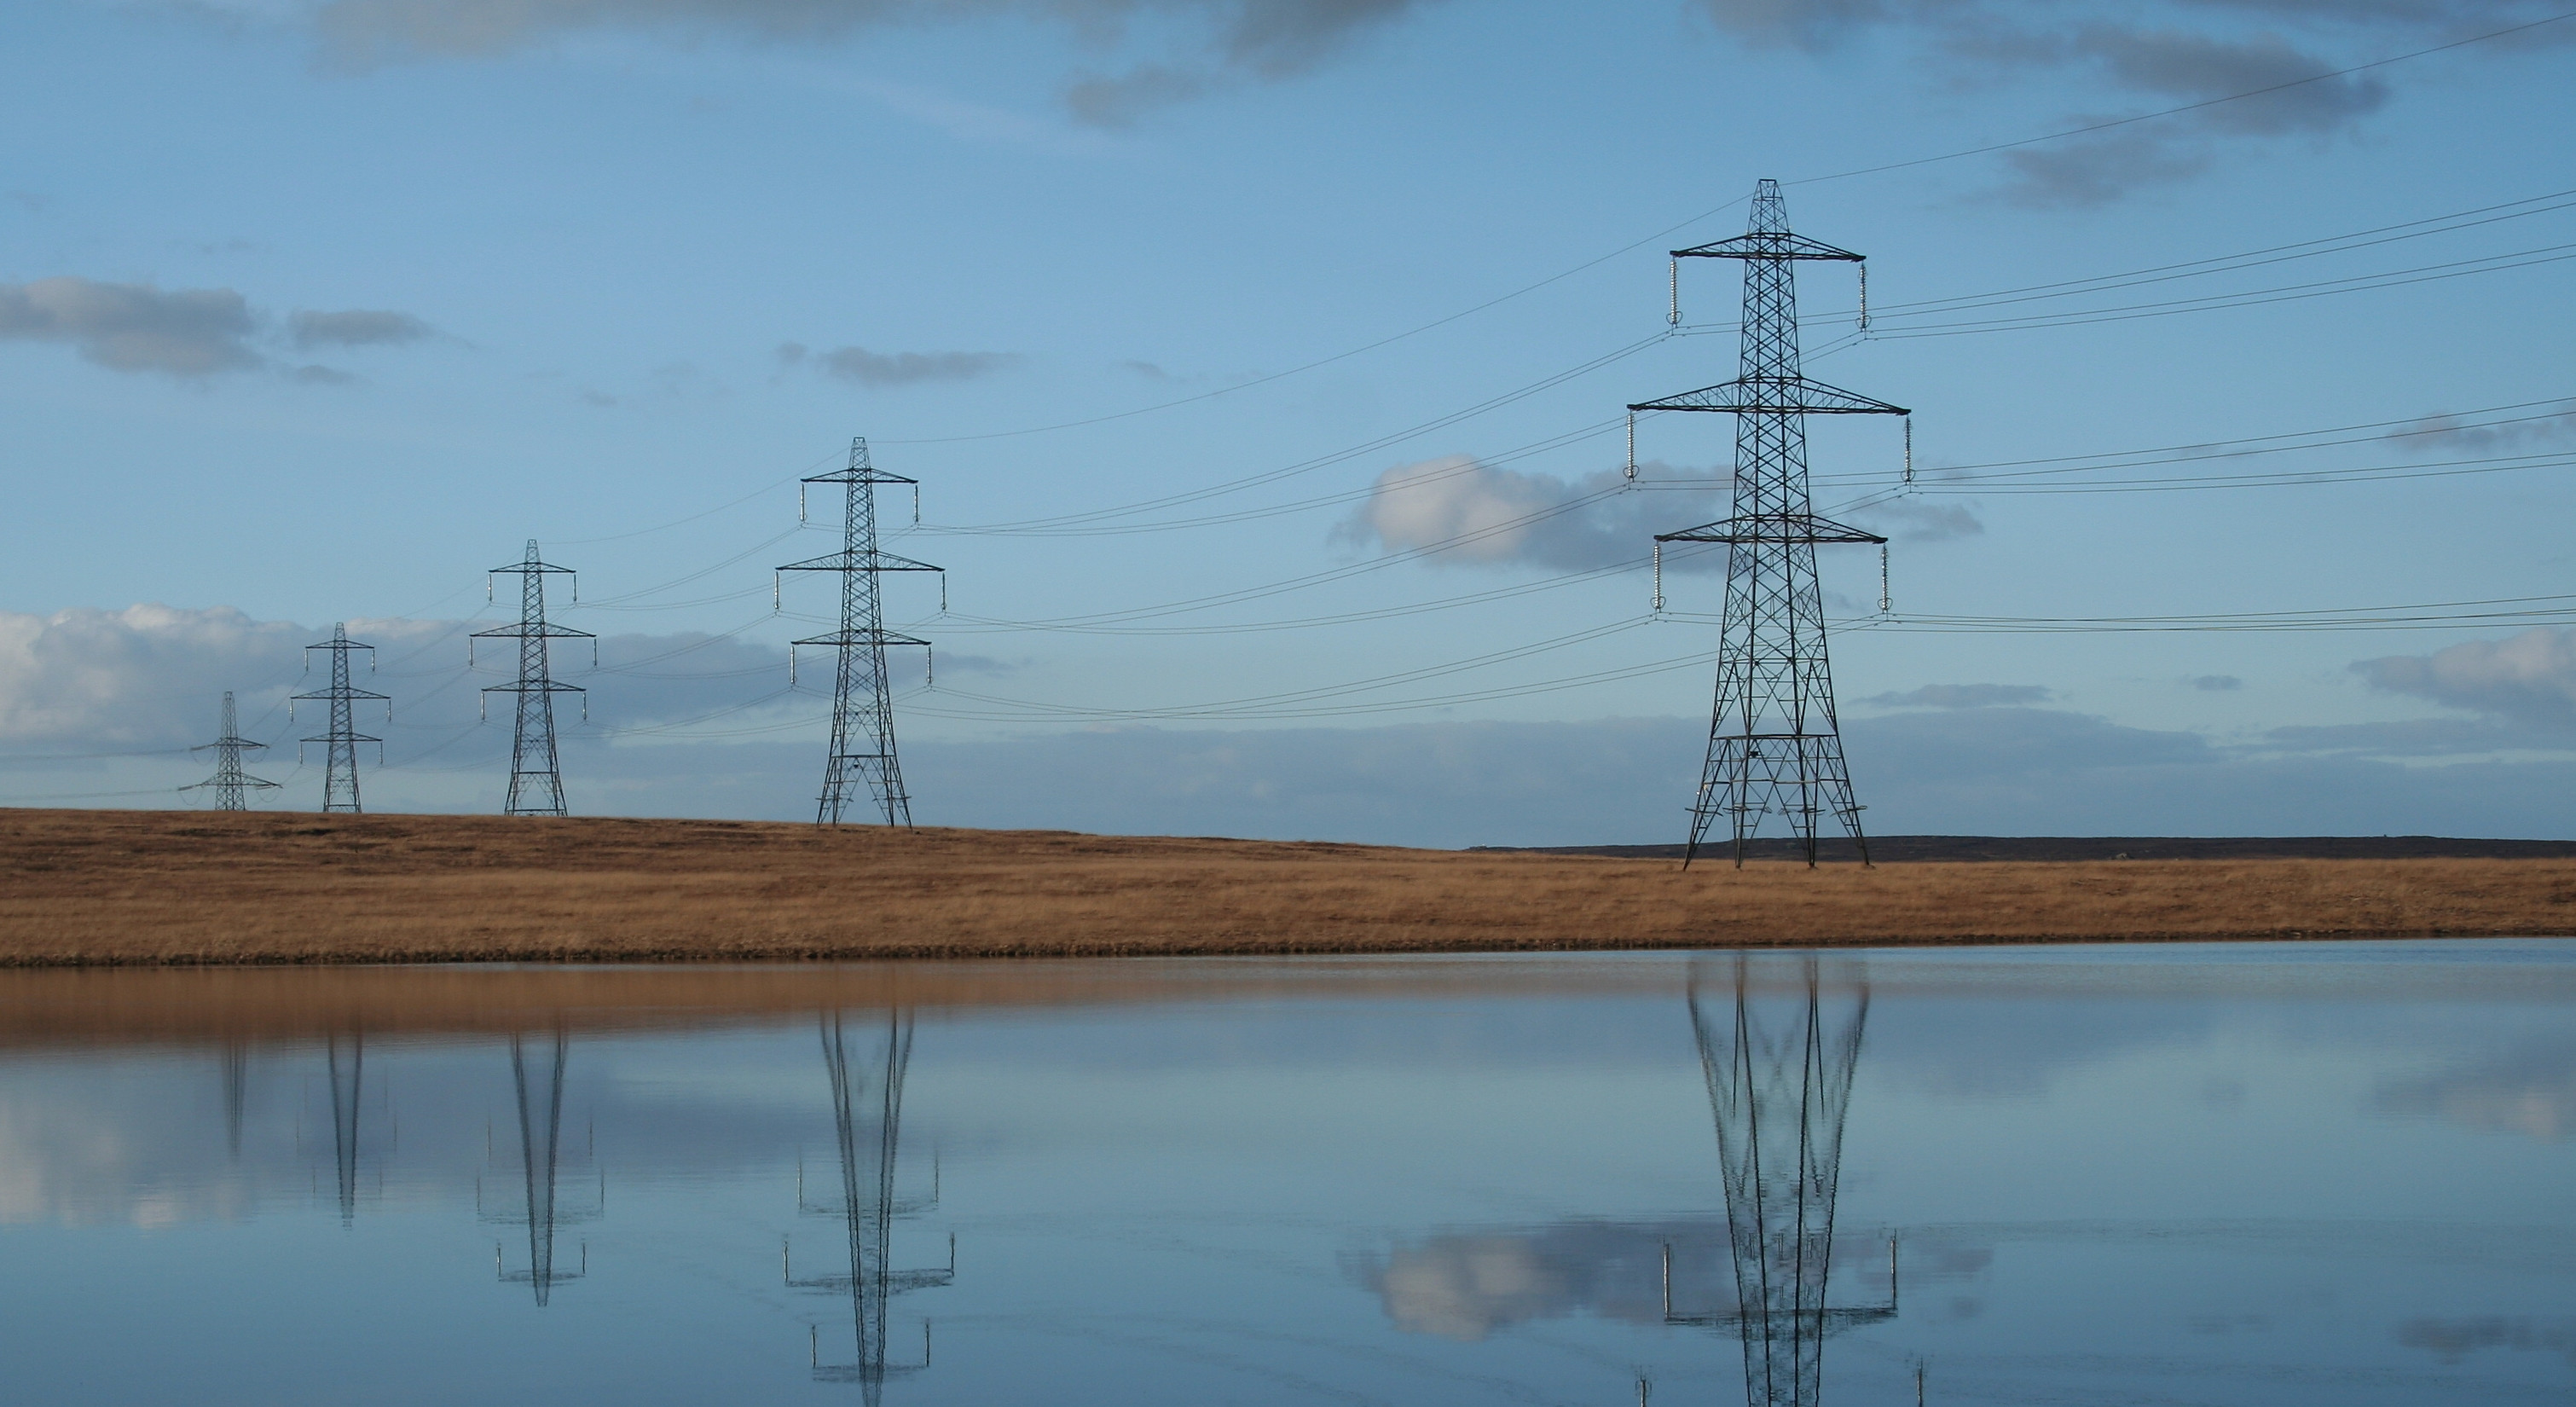
\includegraphics[width=0.7\textwidth]{figures/Pylones_by_Graham_Sivills.jpg} 
 \end{center}

\begin{exercicecours}[Tension minimale]
On se donne deux poteaux distants d'une longueur $2x_0$ fixée et d'une hauteur suffisante.
Parmi toutes les chaînettes passant par les sommets de ces poteaux, on cherche celle
qui a les forces de tensions minimales.

Nous savons que la tension totale (voir la proposition \ref{prop:tens})
vaut 
$$T_x(a) = a \mu g \cdot \ch \frac{x}{a}.$$
Pour une chaînette donnée, la tension est donc maximale au point d'accroche (en $x=x_0$)
car le cosinus hyperbolique est une fonction croissante sur $[0,+\infty[$. Pour un $a$
fixé, la tension maximale est donc $T_{x_0}(a)$. Notre problème, $x_0$ étant fixé, est de trouver
le $a$ qui minimise $T_{x_0}(a)$.
\shorthandoff{:}
\myfigure{1}{
\tikzinput{fig_chainette13}
}
\shorthandon{:}
\begin{enumerate}
 \item Considérations physiques : Que vaut la tension si la chaînette est rectiligne (la longueur de la chaînette
est celle de l'écartement) ? Que vaut la tension si la longueur de la chaînette est infinie ?
%% Dans les deux cas la tension est infinie, cela peut se montrer aussi par les calculs.

 \item Montrer que l'équation $\ch t = t \sh t$ est équivalente à l'équation 
$(t-1)e^{2t}=t+1$. Montrer que, sur $[0,+\infty[$, cette équation a une unique solution $\tau$.
Une valeur approchée de $\tau$ est $\tau = 1,19968\ldots$

%% $f(t) = (t-1)e^{2t}-t-1$, $f'(t) = (2t-1)e^{2t}-1$, $f''(t) = 4te^{2t}$.
% Poutr $t>0$, $f''(t)>0$ donc $f'$ strictement croissante.
% Or $f'(0)=-2$ le limite de $f'$ est $+\infty$ est $+\infty$. 
% Donc $f'$ s'annule en une seule valeur $\tau'$.
% Sur $[0,\tau']$, $f$ est décroissante, sur $[\tau', +\infty[$, $f$ est croissante.
% Comme $f(0) = -2 <0$ il n'y a pas de solution $f(t)=0$ sur $[0,\tau']$.
% Par le théorème des valeurs intermédiaires il existe un unique $\tau \in [\tau', +\infty[$
% tel que $f(\tau)=0$.

 \item Montrer que la tension $T_{x_0}(a)$ est minimale en $a= \frac{x_0}{\tau}$.

% $T'(a) = \mu g \left( \ch\frac{x_0}{a} - \frac{x_0}{a}\sh\frac{x_0}{a} \right)$
% S'annule en $\frac{x_0}{a} = \tau$ uniquement.
% Par les considérations physiques ce point est le minimum !

 \item Calculer la longueur correspondante, ainsi que la flèche.
\shorthandoff{:}
\myfigure{1}{
\tikzinput{fig_chainette14}
}
\shorthandon{:}
% $\ell = a \sh\frac{x_0}{a}  = \frac{x_0}{\tau} \sh \tau$
% $h = a \ch\frac{x_0}{a}  - a = \frac{x_0}{\tau} \ch \tau  - \frac{x_0}{\tau}$

\end{enumerate}

\end{exercicecours}

\medskip



\begin{exercicecours}[Pont suspendu]
Nous allons calculer que la courbe du câble d'un pont suspendu
est une parabole.


Soit le tablier d'un pont de longueur $L$ et de masse totale $M$.
Un gros câble est accroché entre deux pylônes. \`A ce câble sont accrochés
un grand nombre de petits câbles de suspension verticaux reliant le gros câble au tablier.

\shorthandoff{:}
\myfigure{1}{
\tikzinput{fig_chainette15}
}
\shorthandon{:}
Nous allons calculer l'équation $y(x)$ du câble. On s'inspirera pour les premières questions
des calculs sur la chaînette.

\begin{enumerate}

 \item Quelles sont les forces qui s'appliquent à une portion de câble dont l'abscisse est entre
 $x$ et $x+dx$ ?

% Quatre forces : $T(x)$, $-T(x+dx)$, $P(x)$, et la charge $C = Mg/L.dx$ dirigée vers le bas.

 \item \'Ecrire l'équation du principe fondamental de la mécanique, appliqué à cette portion.

% idem chainette + charge 

 \item Montrer que la tension horizontale est indépendante de $x$.

% idem chainette

 \item Montrer que la tension verticale vérifie l'équation différentielle :
$T'_v(x)=-T_h \cdot y''(x)$.

% idem chainette

 \item Dans toute la suite nous supposerons que la masse du câble est négligeable devant
celle du tablier. Cela revient à supposer que le poids $P(x)$ du câble est négligeable devant
la charge $C(x)$ du tablier. Nous posons donc $P(x)=0$.
Montrer que le principe fondamental de la mécanique s'écrit alors :
$$T_h \cdot y''(x) = \frac{M}{L} g.$$

% facile, ressemble chainette

 \item Quelle est l'équation $y(x)$ du câble ?

% Parabole

 \item Calculer une équation du câble du \emph{Golden Bridge} (San Francisco).
Le tablier mesure $1280$ mètres de long, les pylônes ont une hauteur de $160$ mètres (au-dessus
du tablier) et le câble descend jusqu'au tablier (au milieu du pont).

\bigskip

\shorthandoff{:}
\myfigure{1.2}{
\tikzinput{fig_chainette16}
}
\shorthandon{:}


% Repère adapté : unité le mètre, (O,i,j) : O milieu du pont, i horizontal, j vertical.
% y = ax^2+bx + c
% y(0)=0 donc c=0, 
% par symetrie (principe physique) y(-x)=y(x) donc b=0
% y = ax^2 avec a = 160 / (1280/2)^2.
\end{enumerate}

\end{exercicecours}

\bigskip

{\centering 
  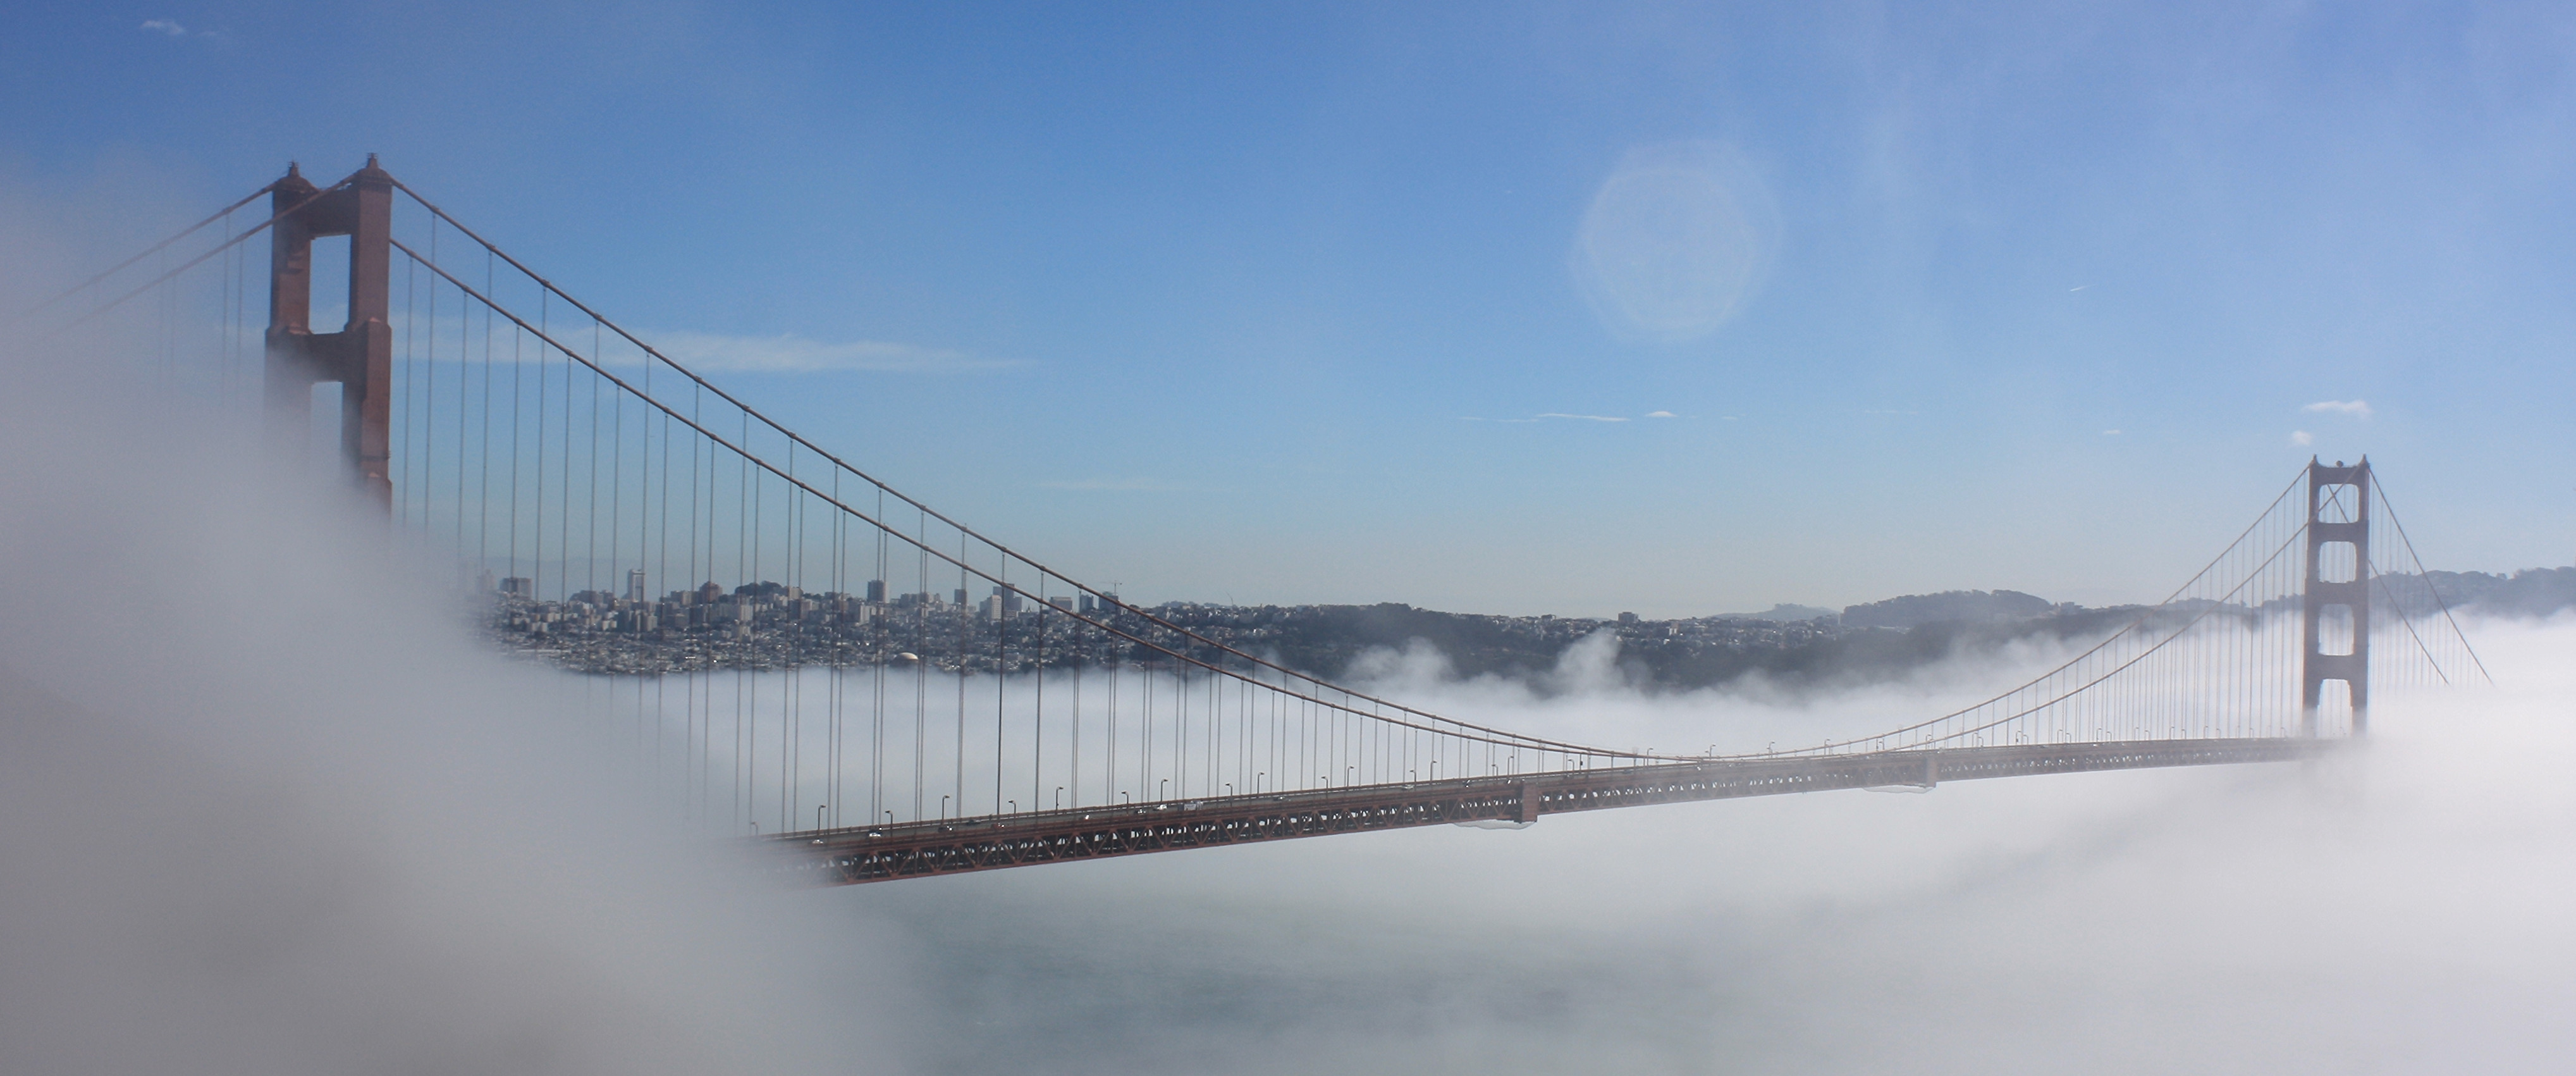
\includegraphics[width=\textwidth]{figures/Golden_Gate_Bridge_by_Mark_Gunn.jpg} 
}

%%%%%%%%%%%%%%%%%%%%%%%%%%%%%%%%%%%%%%%%%%%%%%%%%%%%%%%%%%%%%%%%
%%%%%%%%%%%%%%%%%%%%%%%%%%%%%%%%%%%%%%%%%%%%%%%%%%%%%%%%%%%%%%%%

\bigskip
\bigskip

\auteurs{
Arnaud Bodin

Relu par Laura Desideri.

Photos : fdecomite, soapbubble.dk, N. Jamal, G. Sivills, M. Gunn.
}

\finchapitre
\end{document}

